% Jacob Neumann

% DOCUMENT CLASS AND PACKAGE USE
    \documentclass[aspectratio=169, handout]{beamer}

    % Establish the colorlambda boolean, to control whether the lambda is solid color (true), or the same as the picture (false)
    \newif\ifcolorlambda
    \colorlambdafalse % DEFAULT: false

    % Use auxcolor for syntax highlighting
    \newif\ifuseaux
    \useauxfalse % DEFAULT: false

    % Color settings
    \useauxtrue

    \newcommand{\auxColor}{5725E4}     % the color of note boxes and stuff
    \newcommand{\presentColor}{FABC60} % the primary color of the slide borders
    \newcommand{\bgColor}{fff8ed}      % the color of the background of the slide
    \newcommand{\darkBg}{8b98ad}
    \newcommand{\lambdaColor}{\auxColor}
    \definecolor{auxColor}{HTML}{\auxColor}
    \newcommand{\mygreen}[0]{%
      \color{green!55!black}
    }

    \colorlambdatrue

    \usepackage{comment} % comment blocks
    \usepackage{soul} % strikethrough
    \usepackage{listings} % code
    \usepackage{makecell}

    \setbeamertemplate{itemize items}[circle]
    % \setbeameroption{show notes on second screen=right}

    \usepackage{lectureSlides}
    %%%%%%%%%%%%%%%%%%%%%%%%%%%%%%%%%%%%%%%%%| <----- Don't make the title any longer than this
    \title{Sorting and Parallelism} % TODO
    \subtitle{Multitasking madness} % TODO
    \date{06 June 2023} % TODO
    \author{Brandon Wu} % TODO

    \graphicspath{ {./img/} }
    % DONT FORGET TO PUT [fragile] on frames with codeblocks, specs, etc.
        %\begin{frame}[fragile]
        %\begin{codeblock}
        %fun fact 0 = 1
        %  | fact n = n * fact(n-1)
        %\end{codeblock}
        %\end{frame}

    % INCLUDING codefile:
        % 1. In some file under code/NN (where NN is the lecture id num), include:
    %       (* FRAGMENT KK *)
    %           <CONTENT>
    %       (* END KK *)

    %    Remember to not put anything on the same line as the FRAGMENT or END comment, as that won't be included. KK here is some (not-zero-padded) integer. Note that you MUST have fragments 0,1,...,KK-1 defined in this manner in order for fragment KK to be properly extracted.
        %  2. On the slide where you want code fragment K
                % \smlFrag[color]{KK}
        %     where 'color' is some color string (defaults to 'white'. Don't use presentColor.
    %  3. If you want to offset the line numbers (e.g. have them start at line 5 instead of 1), use
                % \smlFragOffset[color]{KK}{5}

\begin{document}

% Make it so ./mkWeb works correctly
\ifweb
    \renewcommand{\pause}{}
\fi

\setbeamertemplate{itemize items}[circle]

% SOLID COLOR TITLE (see SETTINGS.sty)
{
\begin{frame}[plain]
    \colorlambdatrue
    \titlepage
\end{frame}
}

\begin{frame}[fragile]
  \frametitle{Lesson Plan}

  \tableofcontents
\end{frame}

\begin{frame}[fragile]
  \frametitle{Last time}

  Last time, we reviewed the idea of \term{asymptotic analysis}, which is the analysis
  of the performance of programs, as the input size grows.

  \pause
  \vspace{\fill}

  We learned that for recursive, functional programs, we could write mathematical
  \term{recurrences} that described the \code{work} of the code, and that could be solved
  via the \term{unrolling} method to obtain a closed form, and a bound.

  \pause
  \vspace{\fill}

  We also learned that, by assuming we had infinitely many processors, we could
  obtain recurrences that measured the \code{span} of the code, or the amount of time
  using parallelism. We saw that this gave performance benefits for \code{treesum} on
  balanced trees.
\end{frame}

\sectionSlide{1}{Analyzing a Tree via Depth}

\begin{frame}[fragile]
  \frametitle{Measuring a Tree (again)}

  Before, we discussed how we could use the number of nodes in a tree as the input
  size, and obtain two span recurrences for \code{treesum} -- $O(n)$ in the imbalanced
  case, and $O(\log n)$ in the balanced case.

  \pause
  \vspace{\fill}

  That's not the only way to measure a tree, though.\footnote{You can also use a tape measure.} The other way is that we could
  use the \term{depth} of the tree, which is the longest path through the tree to
  get to the bottom.

  \pause
  \vspace{\fill}

  \begin{codeblock}
    fun treesum (Empty : tree) : int = 0
      | treesum (Node (L, x, R)) = treesum L + x + treesum R
  \end{codeblock}

  \vspace{\fill}

  Let's try it!
\end{frame}

\begin{frame}[fragile]
  \frametitle{Tree Recurrence: Depth}

  Where $d$ is the depth of the tree \code{T}, in the expression \code{treesum T}:
  $$S_{\code{treesum}}(0) = c_0$$
  $$S_{\code{treesum}}(d) = \max(S_{\code{treesum}}(d_{\code{L}}), c_1, S_{\code{treesum}}(d_{\code{R}})) + c_2\footnote{
    Recall that the $c_1$ term is obtained via the constant amount
    of work involved in the computation of \code{x}. It's already a value, but
    there is \textit{some} constant work associated, and we do take the max over it,
    in case it unexpectedly takes a really long time.\footnotemark
  }$$

  \pause
  \vspace{\fill}

  Again, we don't know how deep the tree is in the left and right subtrees --
  our recurrence depends on the quantities $d_{\code{L}}$ and $d_{\code{R}}$,
  respectively.

  \pause
  \vspace{\fill}

  We find ourselves in the same situation as before, and we'll solve it the same
  way, by assuming the worst case. In the worst case, the tree is just a spine,
  so the depth of the left is $d - 1$, and the depth of the right is $0$.

  \footnotetext[3]{It doesn't.}
\end{frame}

\begin{frame}[fragile]
  \frametitle{Tree Recurrence: Depth (Unbalanced)}

  \customBox{Case}{\, The \textbf{span} of \code{treesum} on an \textbf{unbalanced} tree, in terms of the \textbf{depth} $d$.}
  $$S_{\code{treesum}}(d) = \max(S_{\code{treesum}}(d - 1), c_1, S_{\code{treesum}}(0)) + c_2$$
  $$S_{\code{treesum}}(d) = S_{\code{treesum}}(d - 1) + c_2$$

  \pause
  \vspace{\fill}

  If we exchange $d$ for $n$, we've seen this recurrence before. This solves to $O(d)$.
  \begin{align*}
    & S_{\code{treesum}}(d) \\
    &= S_{\code{treesum}}(d - 1) + c_2 \\
    &= S_{\code{treesum}}(d - 2) + c_2 + c_2 \\
    &= ... \\
    &= \sum_{i = 1}^d c_2 + c_0 \\
    &= d \cdot c_2 + c_0
  \end{align*}
\end{frame}

\begin{frame}[fragile]
  \frametitle{Tree Recurrence: Depth (Balanced)}

  \customBox{Case}{\, The \textbf{span} of \code{treesum} on a \textbf{balanced} tree, in terms of the \textbf{depth} $d$.}

  \pause
  \vspace{\fill}

  Then, the left subtree still has depth $d - 1$, as does the
  right subtree.

  \pause
  \vspace{\fill}

  So:
  $$S_{\code{treesum}}(d) = \max(S_{\code{treesum}}(d - 1), c_1, S_{\code{treesum}}(d - 1)) + c_2$$
  $$S_{\code{treesum}}(d) = S_{\code{treesum}}(d - 1) + c_2$$

  \pause
  \vspace{\fill}

  What gives?? This is the same recurrence! Span is $O(d)$ in both the unbalanced and
  balanced cases.
\end{frame}

\begin{frame}[fragile]
  \frametitle{On Depth and Balance}

  This might be counterintuitive, because we expect a better bound, but it makes sense if
  you remember the task dependency graphs we discussed earlier.

  \pause
  \vspace{\fill}

  In a task dependency graph, the cost of executing some amount of tasks in parallel is
  just the \textit{longest path through the graph}, or tree. The length of the longest
  path through a tree is just $d$, the depth of the tree, because a tree has the
  structure of a dependency graph that is just the same tree!

  \pause
  \vspace{\fill}

  We can relate it back to our previous bounds, $O(n)$ and $O(\log n)$, for unbalanced and
  balanced trees, in the number of nodes $n$, however.
\end{frame}

\begin{frame}[fragile]
  \frametitle{On Depth and Balance}

  \ptmt

  \keyBox{}{ In an unbalanced tree, the depth $d$ is just the number of nodes $n$.}

  \pause
  \vspace{\fill}

  So in the unbalanced case, an $O(d)$ bound is the same as $O(n)$, which is the same
  bound we received earlier.

  \pause
  \vspace{\fill}

  What is the number of nodes in a balanced tree of depth $d$ though? Well, each level has
  double the nodes of the previous, so it's equal to
  $$1 + 2 + 4 + ... + 2^d$$

  \pause
  \vspace{\fill}

  \keyBox{}{ There's a lovely geometric proof that shows that this is in $O(2^d)$.}

  \pause
  \vspace{\fill}

  So in a balanced tree, $n \approx 2^d$, so our previous bound is $O(\log n) = O(\log (2^d)) = O(d)$.
  We get the same thing either way, so this is perfectly consistent!
\end{frame}

\begin{frame}[fragile]
  \frametitle{A Picture Proof}

  \begin{center}
    \begin{tikzpicture}[scale=2.25]
      % Draw the outer square
      \draw (0, 0) rectangle (2, 2);
      \node (A) at (0.5,1) {$n$};

      % Draw the rectangles inside
      \draw (1, 0) -- (1, 2);
      \node (A) at (1.5,1.5) {\Large $\frac{n}{2}$};

      % Draw the squares inside
      \draw (1, 1) -- (2, 1);
      \node (A) at (1.75, 0.5) {\Large $\frac{n}{4}$};

      \draw (1.5, 0) -- (1.5, 1);
      \node (A) at (1.25,0.25) {\Large $\frac{n}{8}$};

      \draw (1, 0.5) -- (1.5, 0.5);
      \node (A) at (1.25,0.75) {\Large \textellipsis};
    \end{tikzpicture}
  \end{center}

  \pause
  \vspace{\fill}

  We can see that if we do an infinite sum of $n + \frac{n}{2} + \frac{n}{4} + ...$,
  the sum never surpasses the area of the square, which is just twice of the left half,
  otherwise known as $2n$.

  \pause
  \vspace{\fill}

  Since the finite sum $1 + 2 + 4 + ... + n$ is definitely smaller than this, we are
  fine to conclude that it is on the order of $O(n)$.
\end{frame}


\begin{frame}[fragile]
  \frametitle{Nodes or Depth}

  Ultimately, if you do the math and reason it out, you find that getting bounds in terms of
  depth and nodes looks different, but ultimately say the same thing.

  \pause
  \vspace{\fill}

  Whichever is "easier" is up to your discretion. Both are valid ways of solving a
  recurrence.\footnote{
    We will usually specify whenever we have a particular way we want to
    see you solve it, which is often.
  }

  \pause
  \vspace{\fill}

  \begin{center}
    \begin{tabular}{ c|c|c }
    Span of \code{treesum} & Nodes & Depth \\
    \hline & \\[-1.5ex]
     Balanced & $O(\log n)$ & $O(d)$ \\ [0.5ex]
    \hline & \\[-1.5ex]
     Unbalanced & $O(n)$ & $O(d)$
    \end{tabular}
  \end{center}

\end{frame}

\sectionSlide{2}{The Tree Method}

% TODO: move this to lecture6, move parallelism stuff here?
% actually, inclined to keep it this way, i think...
\begin{frame}[fragile]
  \frametitle{Ordering a Tree}

  Recall our notion of an \textit{traversal} on a tree, which produces
  a list from a tree by traversing the tree in some prescribed order.

  \pause
  \vspace{\fill}

  We are interested in \textit{inorder} traversal, which traverses a
  tree the same way that someone would traverse it by reading from
  left-to-right.

  \pause
  \vspace{\fill}

  \begin{codeblock}
    fun inord (Empty : tree) : int list = []
      | inord (Node (L, x, R)) = inord L @ (x :: inord R)
  \end{codeblock}
\end{frame}

\begin{frame}[fragile]
  \frametitle{\code{inord}, Naively}

  When you see recursive calls being given as arguments to append, you
  should double-check, because something fishy is probably going on.

  \pause
  \vspace{\fill}

  But, better than thinking about it, we can mathematically solve for the
  performance! Let's assume a balanced tree, and solve for the work of this
  function, in terms of the nodes of the tree.

  \pause
  \vspace{\fill}

  \customBox{Case}{\, The \textbf{work} of \code{inord} on a \textbf{balanced} tree.}

  \pause
  \vspace{\fill}

  Where $n$ is the number of nodes in the input tree:
  $$W_{\code{inord}}(0) = c_0$$
  $$W_{\code{inord}}(n) = c_1 + W_{\code{@}}\left(\frac{n}{2}\right) + 2 \cdot W_{\code{inord}}\left(\frac{n}{2}\right)$$

  (because we append a list of half the size, and compute \code{inord} recursively twice)
\end{frame}

\begin{frame}[fragile]
  \frametitle{Solving \code{inord}}

  So we have:
  \begin{align*}
    & W_{\code{inord}}(n) \\
    &= c_1 + W_{\code{@}}\left(\frac{n}{2}\right) + 2 \cdot W_{\code{inord}}\left(\frac{n}{2}\right) \\
    &= c_1 + O(n)  + 2 \cdot W_{\code{inord}}\left(\frac{n}{2}\right) \\
    &= c_1 + O(n) + 2 \cdot \left(c_1 + O\left(\frac{n}{4}\right) + 2 \cdot W_{\code{inord}}\left(\frac{n}{4}\right)\right) \\
    &= c_1 + O(n) + 2 \cdot \left(c_1 + O\left(\frac{n}{4}\right) + 2 \cdot \left(c_1 + O\left(\frac{n}{8}\right) + 2 \cdot W_{\code{inord}}\left(\frac{n}{8}\right)\right)\right) \\
    &= ... = \, ???
  \end{align*}

  \pause
  This is... messy.\footnote{Life is, sometimes.}
\end{frame}

\begin{frame}[fragile]
  \frametitle{Unrolling in the Deep}

  Sometimes, unrolling is messy. Sometimes, like in \code{length}, we only get
  one extra term per "unrolling", and so it's not hard to solve by just
  finding the pattern.

  \pause
  \vspace{\fill}

  In the case of functions on trees, this usually isn't the case! We actually
  get \textit{two} terms per unrolling, which quickly becomes four by the
  next unrolling, and so on. This is much harder to eyeball.

  \pause
  \vspace{\fill}

  We will employ a new technique of solving for such recurrences, using the
  \term{tree method}, instead of the unrolling method.
\end{frame}

\begin{frame}[fragile]
  \frametitle{The Tree Method}

  \rprs

  The tree method gets its name, from noticing that the amount of recursive
  calls done by a function like \code{inord} induces a tree structure.

  \pause
  \vspace{\fill}

  We see that calling \code{inord} on a tree with $n$ nodes causes two
  calls, to \code{inord} with $\frac{n}{2}$ nodes (in the balanced case).

  \pause
  \vspace{\fill}

  So let's draw a tree representing the computation of \code{inord T}, with nodes
  annotated with the size of the input at each call, with edges indicating
  recursive calls:

  \pause
  \vspace{\fill}

  \makebox[\textwidth][c]{
    \begin{tikzpicture}
      \node[shape=circle,draw=black] (T) at (2,4) { $n$} ;

      \node[shape=circle,draw=black] (M1) at (-1,2.5) { $\frac{n}{2}$};
      \node[shape=circle,draw=black] (M2) at (5,2.5) { $\frac{n}{2}$};

      \draw[->] (T) -- (M1);
      \draw[->] (T) -- (M2);
  \end{tikzpicture}
  }

\end{frame}

\begin{frame}[fragile]
  \frametitle{Tree Call Structure}

  But those two calls to \code{inord} have their own recursive calls,
  which have size $\frac{n}{4}$.

  So our "call tree" expands to:

  \pause
  \makebox[\textwidth][c]{
    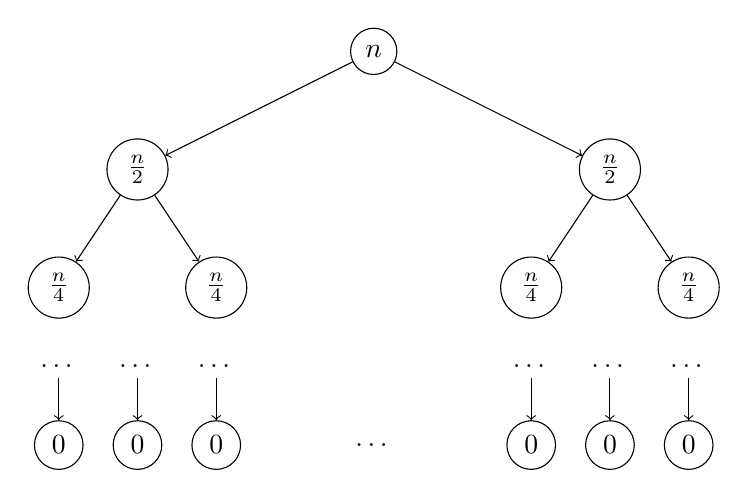
\begin{tikzpicture}
      \node[shape=circle,draw=black] (T) at (2,4) { $n$} ;

      \node[shape=circle,draw=black] (M1) at (-1,2.5) { $\frac{n}{2}$};
      \node[shape=circle,draw=black] (M2) at (5,2.5) { $\frac{n}{2}$};

      \node[shape=circle,draw=black] (L1) at (-2,1) { $\frac{n}{4}$};
      \node[shape=circle,draw=black] (L2) at (0,1) { $\frac{n}{4}$};

      \node[shape=circle,draw=black] (L3) at (4,1) { $\frac{n}{4}$};
      \node[shape=circle,draw=black] (L4) at (6,1) { $\frac{n}{4}$};

      \node[shape=circle,draw=black] (LL1) at (-2,-1) { $0$};
      \node[shape=circle,draw=black] (LL2) at (-1,-1) { $0$};
      \node[shape=circle,draw=black] (LL3) at (0,-1) { $0$};

      \node[shape=circle,draw=black] (LL4) at (4,-1) { $0$};
      \node[shape=circle,draw=black] (LL5) at (5,-1) { $0$};
      \node[shape=circle,draw=black] (LL6) at (6,-1) { $0$};

      \node[] (LLM) at (2,-1) { \textellipsis};

      \node [above of=LL1] (ULL1) {\textellipsis};
      \node [above of=LL2] (ULL2) {\textellipsis};
      \node [above of=LL3] (ULL3) {\textellipsis};
      \node [above of=LL4] (ULL4) {\textellipsis};
      \node [above of=LL5] (ULL5) {\textellipsis};
      \node [above of=LL6] (ULL6) {\textellipsis};

      \draw[->] (T) -- (M1);
      \draw[->] (T) -- (M2);

      \draw[->] (M1) -- (L1);
      \draw[->] (M1) -- (L2);
      \draw[->] (M2) -- (L3);
      \draw[->] (M2) -- (L4);

      \draw[->] (ULL1) -- (LL1);
      \draw[->] (ULL2) -- (LL2);
      \draw[->] (ULL3) -- (LL3);
      \draw[->] (ULL4) -- (LL4);
      \draw[->] (ULL5) -- (LL5);
      \draw[->] (ULL6) -- (LL6);
  \end{tikzpicture}
  }
\end{frame}

\begin{frame}[fragile]
  \frametitle{Tree Call Structure}

  \ptmt

  We can think of the following recurrence as three parts:
  \pause
  $$W_{\code{inord}}({\color{green!55!black} n}) = {\color{auxColor} c_1 + W_{\code{@}}(\frac{n}{2})} + {\color{red} 2 \cdot W_{\code{inord}}(\frac{n}{2})}$$

  \pause
  \begin{itemize}
    \item the \textit{nonrecursive work}, ${\color{auxColor} W_{\code{@}}(\frac{n}{2}) + c_1}$ \pause
    \item the \textit{recursive work}, ${\color{red} 2 \cdot W_{\code{inord}}(\frac{n}{2})}$ \pause
    \item for a given \textit{input size}, which is ${\color{green!55!black}n}$
  \end{itemize}

  \pause
  \vspace{\fill}

  With respect to the call tree, the nonrecursive work is the work present at each
  node, but the recursive work is taken care of by all its children.

  \pause
  \vspace{\fill}

  So, if we sum all the nonrecursive work in \textbf{each node}, we'll get the work
  done by the entire function.
\end{frame}

\begin{frame}[fragile]
  \frametitle{The Work of a Node}

  $$W_{\code{inord}}({\color{green!55!black} n}) = {\color{auxColor} c_1 + W_{\code{@}}(\frac{n}{2})} + {\color{red} 2 \cdot W_{\code{inord}}(\frac{n}{2})}$$

  \pause
  \vspace{\fill}

  To do this, we'll need to somehow figure out the nonrecursive work
  done by each node. This is $O(n) + c_1$ for a node with size ${\mygreen n}$,
  except each node has a different size!

  \pause
  \vspace{\fill}

  In addition, there's a differing number of nodes of each size,
  since there's 2 of size ${\mygreen \frac{n}{2}}$, and 4 of size ${\mygreen \frac{n}{4}}$,
  and so on.

  \pause
  \vspace{\fill}

  This isn't easier at all!
\end{frame}

\begin{frame}[fragile]
  \frametitle{Get On My Level}

  The innovation comes from noticing that the nonrecursive work
  at each \textit{level} of the tree might come out to the same thing.

  \pause
  \vspace{\fill}

  If the work at each level was the same, then we could just multiply
  that quantity by the height of the tree, which is $\log n$, the number
  of times we can recursively call \code{inord} by halving the input.

  \pause
  \vspace{\fill}

  Let's try it out.
\end{frame}

\begin{frame}[fragile]
  \frametitle{\code{inord}: Tree Call Structure}

  \makebox[\textwidth][c]{
    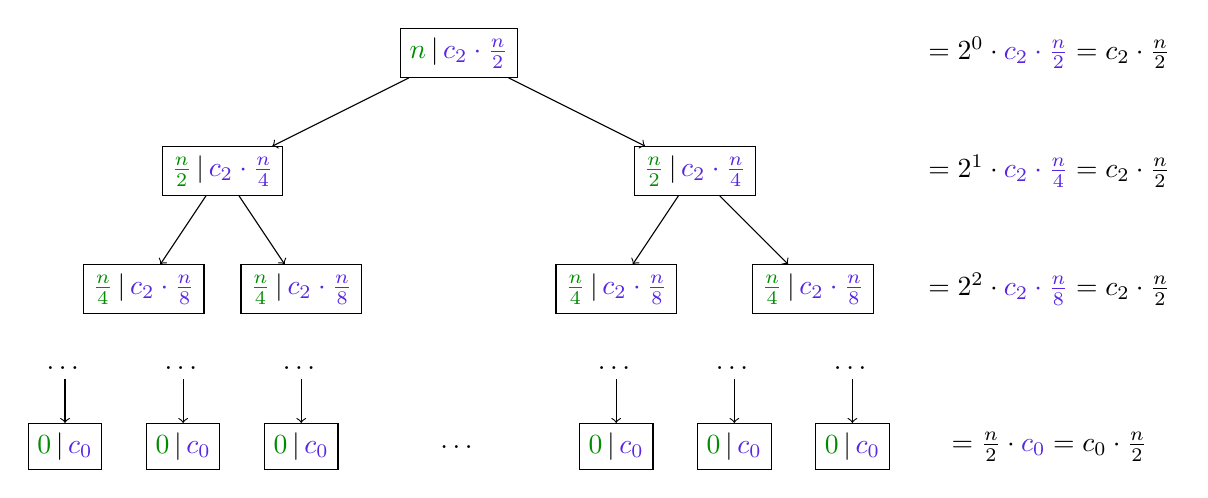
\begin{tikzpicture}
      \node[shape=rectangle,draw=black] (T) at (2,4) { ${\mygreen n} \, \vert \,  {\color{auxColor} c_2 \cdot \frac{n}{2}}$ } ;

      \node[shape=rectangle,draw=black] (M1) at (-1,2.5) { ${ \mygreen \frac{n}{2}} \, \vert \, {\color{auxColor} c_2 \cdot \frac{n}{4}}$};
      \node[shape=rectangle,draw=black] (M2) at (5, 2.5) { ${ \mygreen \frac{n}{2}} \, \vert \, {\color{auxColor} c_2 \cdot \frac{n}{4}}$};

      \node[shape=rectangle,draw=black] (L1) at (-2,1) { ${ \mygreen \frac{n}{4}} \, \vert \, {\color{auxColor} c_2 \cdot \frac{n}{8}}$};
      \node[shape=rectangle,draw=black] (L2) at (0,1) { ${ \mygreen \frac{n}{4}} \, \vert \, {\color{auxColor} c_2 \cdot \frac{n}{8}}$};

      \node[shape=rectangle,draw=black] (L3) at (4,1) { ${ \mygreen \frac{n}{4}} \, \vert \, {\color{auxColor} c_2 \cdot \frac{n}{8}}$};
      \node[shape=rectangle,draw=black] (L4) at (6.5,1) { ${ \mygreen \frac{n}{4}} \, \vert \, {\color{auxColor} c_2 \cdot \frac{n}{8}}$};

      \node[shape=rectangle,draw=black] (LL1) at (-3,-1) { ${\mygreen 0} \, \vert \, {\color{auxColor} c_0}$};
      \node[shape=rectangle,draw=black] (LL2) at (-1.5,-1) { ${\mygreen 0} \, \vert \, {\color{auxColor} c_0}$};
      \node[shape=rectangle,draw=black] (LL3) at (0, -1) { ${\mygreen 0} \, \vert \, {\color{auxColor} c_0}$};

      \node[shape=rectangle,draw=black] (LL4) at (4,-1) { ${\mygreen 0} \, \vert \, {\color{auxColor} c_0}$};
      \node[shape=rectangle,draw=black] (LL5) at (5.5,-1) { ${\mygreen 0} \, \vert \, {\color{auxColor} c_0}$};
      \node[shape=rectangle,draw=black] (LL6) at (7, -1) { ${\mygreen 0} \, \vert \, {\color{auxColor} c_0}$};

      %\node[] (D1) at (-5, 4) { $= 2^0 \cdot {\color{auxColor} c_2 \cdot \frac{n}{2}} = c_1 \cdot \frac{n}{2}$ };
      %\node[] (D2) at (-5, 1) { $= 2^1 \cdot {\color{auxColor} c_2 \cdot \frac{n}{2}} = c_1 \cdot \frac{n}{2}$ };
      %\node[] (D3) at (-5, -1) { $= 2^2 \cdot {\color{auxColor} c_2 \cdot \frac{n}{2}} = c_1 \cdot \frac{n}{2}$ };

      \node[] (S1) at (9.5, 4) { $= 2^0 \cdot {\color{auxColor} c_2 \cdot \frac{n}{2}} = c_2 \cdot \frac{n}{2}$ };
      \node[] (S2) at (9.5, 2.5) { $= 2^1 \cdot {\color{auxColor} c_2 \cdot \frac{n}{4}} = c_2 \cdot \frac{n}{2}$ };
      \node[] (S3) at (9.5, 1) { $= 2^2 \cdot {\color{auxColor} c_2 \cdot \frac{n}{8}} = c_2 \cdot \frac{n}{2}$ };
      \node[] (S4) at (9.5, -1) { $= \frac{n}{2} \cdot {\color{auxColor} c_0} = c_0 \cdot \frac{n}{2}$ };

      \node[] (LLM) at (2,-1) { \textellipsis};

      \node [above of=LL1] (ULL1) {\textellipsis};
      \node [above of=LL2] (ULL2) {\textellipsis};
      \node [above of=LL3] (ULL3) {\textellipsis};
      \node [above of=LL4] (ULL4) {\textellipsis};
      \node [above of=LL5] (ULL5) {\textellipsis};
      \node [above of=LL6] (ULL6) {\textellipsis};

      \draw[->] (T) -- (M1);
      \draw[->] (T) -- (M2);

      \draw[->] (M1) -- (L1);
      \draw[->] (M1) -- (L2);
      \draw[->] (M2) -- (L3);
      \draw[->] (M2) -- (L4);

      \draw[->] (ULL1) -- (LL1);
      \draw[->] (ULL2) -- (LL2);
      \draw[->] (ULL3) -- (LL3);
      \draw[->] (ULL4) -- (LL4);
      \draw[->] (ULL5) -- (LL5);
      \draw[->] (ULL6) -- (LL6);
  \end{tikzpicture}
  }

  \vspace{\fill}

  where {\mygreen the green} denotes the size of the input at a node, and {\color{auxColor} the purple}
  denotes the amount of nonrecursive work at that call
\end{frame}

\begin{frame}[fragile]
  \frametitle{The Tree Method, Concluded}

  Let the \textit{level} of a tree denote how far we are from the root.
  So the root is at level $0$, and there are two nodes at level $1$, and
  so on.

  \pause
  \vspace{\fill}

  \customBox{Number of levels}{\, $\log n$, the number of times we can divide the input
  size by $2$}

  \pause
  \vspace{\fill}

  \customBox{Work per node at level $i$}{\, ${\color{auxColor}\dfrac{n}{2^{i + 1}}c_2}$}

  \pause
  \vspace{\fill}

  \customBox{Number of nodes at level $i$}{\, $2^i$}

  \pause
  \vspace{\fill}

  So to solve for our cumulative work at level $i$, we multiply the number of nodes and work per node:
  $$2^i \cdot \left(\dfrac{n}{2^{i + 1}}c_2\right) = \frac{n}{2} \cdot c_2$$

  \pause
  So the work at level $i$, cumulatively, is the same! What's more, it's in $O(n)$.
  There's $\log n$ levels, so we ultimately come out with a bound of
  $O(n \log n)$. \footnote{There are several things we elided to come to this bound. We decided to
  count the nonrecursive work at each node as the work of asymptotically dominating
  \code{@} and we ignored the $c_0$ leaf terms, because they are ultimately
  dominated by the sum of the other layers. We only care about getting to the right asymptotic
  bound, so we can make things disappear if they aren't relevant. }

\end{frame}

\begin{frame}[fragile]
  \frametitle{The \code{inord} Matrix}

  \begin{center}
    \begin{tabular}{ c|c|c }
    Complexity of \code{inord} & Work & Span \\
    \hline & \\[-1.5ex]
     Balanced & $O(n \log n)$ & TBD \\ [0.5ex]
    \hline & \\[-1.5ex]
     Unbalanced & TBD & TBD
    \end{tabular}
  \end{center}

  \pause
  \vspace{\fill}

  So now we've filled in one entry for our matrix of work and span for
  the \code{inord} function, in the balanced and unbalanced case.

  \pause
  \vspace{\fill}

  Let's quickly reason about the unbalanced case for the work.
\end{frame}

\begin{frame}[fragile]
  \frametitle{\code{inord}: Work (Unbalanced)}

  \customBox{Case}{\, The \textbf{work} of \code{inord} on an \textbf{unbalanced} tree.}

  \pause
  \vspace{\fill}

  The worst case would be if the subtree \code{L} had $n - 1$ nodes, in other words
  a left spine. This is because we would have to do an append of $n - 1$ elements.

  \pause
  \vspace{\fill}

  Where $n$ is the number of nodes in the input tree:
  $$ W_{\code{inord}}(0) = c_0 $$
  $$ W_{\code{inord}}(n) = c_1 + W_{\code{@}}(n - 1) + W_{\code{inord}}(n - 1) + W_{\code{inord}}(0)$$

  \vspace{\fill}

  This looks very similar to our \code{rev} recurrence from last lecture. We will
  skip the derivation and conclude that the complexity is $O(n^2)$.
\end{frame}

\begin{frame}[fragile]
  \frametitle{\code{inord}: Span (Balanced)}

  \customBox{Case}{\, The \textbf{span} of \code{inord} on a \textbf{balanced} tree.}

  \vspace{\fill}

  \begin{codeblock}
    fun inord (Empty : tree) : int list = []
      | inord (Node (L, x, R)) = inord L @ (x :: inord R)
  \end{codeblock}

  \pause
  \vspace{\fill}

  Here, we can do the calls to \code{inord L} and \code{inord R} in parallel,
  so we get the same recurrence as the balanced work case, but with only one
  recursive call.

  \pause
  \vspace{\fill}

  Where $n$ is the number of nodes in the input tree:
  $$ S_{\code{inord}}(0) = c_0 $$
  $$ S_{\code{inord}}(n) = \max\left(S_{\code{inord}}\left(\frac{n}{2}\right), c_1,
  S_{\code{inord}}\left(\frac{n}{2}\right)\right) + S_{\code{@}}\left(\frac{n}{2}\right) + c_2$$

\end{frame}

\begin{frame}[fragile]
  \frametitle{\code{inord}: Span (Balanced)}

  \begin{align*}
    & S_{\code{inord}}(n) \\
    &= \max\left(S_{\code{inord}}\left(\frac{n}{2}\right), c_1,
      S_{\code{inord}}\left(\frac{n}{2}\right)\right) + S_{\code{@}}\left(\frac{n}{2}\right) + c_2 \\
    &= S_{\code{inord}}\left(\frac{n}{2}\right) + \frac{n}{2} c_1 + c_2 \\
    &= S_{\code{inord}}\left(\frac{n}{4}\right) + \frac{n}{4} c_1 + c_2 +  \frac{n}{2} c_1 + c_2 \\
    &= ... \\
    &= \sum_{i = 1}^{\log n} \left(\frac{n}{2^i} c_1\right) + \log n \cdot c_2 + \frac{n}{2} c_0
  \end{align*}

  \pause
  \vspace{\fill}

  The first term dominates, because it's $(1 + 2 + 4 + 8 + ... + \frac{n}{2}) c_1$, so we get
  $O(n)$.
\end{frame}

\begin{frame}[fragile]
  \frametitle{The \code{inord} Matrix}

  \begin{center}
    \begin{tabular}{ c|c|c }
    Complexity of \code{inord} & Work & Span \\
    \hline & \\[-1.5ex]
     Balanced & $O(n \log n)$ & $O(n)$ \\ [0.5ex]
    \hline & \\[-1.5ex]
     Unbalanced & $O(n^2)$ & $O(n^2)$
    \end{tabular}
  \end{center}

  \pause
  \vspace{\fill}

  We leave it as an exercise to the reader that the span of the unbalanced
  \code{inord} case is $O(n^2)$.

  \pause
  \vspace{\fill}

  Recall that appending recursive calls typically denotes something fishy.
  Let's try to think and see if we can eliminate that, in favor of a better
  work complexity than $O(n \log n)$.
\end{frame}

\questionBreak{1581 0813}

\quizBreak{\textlangle obfuscated\textrangle}

\sectionSlide{3}{A Better \code{inord}}

\begin{frame}[fragile]
  \frametitle{A Better \code{inord}}

  Let's do \code{inord} again, but this time with an accumulator argument. Let's
  try to avoid using \code{@} with a recursive call.

  \pause
  \vspace{\fill}

  \begin{codeblock}
    fun inord' (Empty : tree, acc : int list) = acc
      | inord' (Node (L, x, R), acc) =
          inord' (L, x :: inord' (R, acc))
  \end{codeblock}

  \pause
  \vspace{\fill}

  Theoretically, the complexity should be better. Let's figure it out!
\end{frame}

\begin{frame}[fragile]
  \frametitle{\code{inord'}: Work (Balanced)}

  \customBox{Case}{\, The \textbf{work} of \code{inord'} on a \textbf{balanced} tree.}

  \pause
  \vspace{\fill}

  Where $n$ is the number of nodes in \code{T} in the expression \code{inord' (T, L)}:
  $$W_{\code{inord'}}(0) = c_0$$
  $$W_{\code{inord'}}(n) = 2 \cdot W_{\code{inord'}}\left(\frac{n}{2}\right) + c_1$$

  \pause
  \vspace{\fill}

  We get two calls to $W_{\code{inord'}}\left(\dfrac{n}{2}\right)$, because we first compute
  \code{inord'(R, acc)}, and then pass that in as \code{acc'} to \code{inord' (L, x :: acc')}.

  \pause
  \vspace{\fill}

  In either case, the size of the tree being called on is roughly half.
\end{frame}

\begin{frame}[fragile]
  \frametitle{\code{inord'}: Work (Balanced)}

  So we solve to:

  \pause
  \begin{align*}
    &= W_{\code{inord'}}(n) \\
    &= 2 \cdot W_{\code{inord'}}(\frac{n}{2}) + c_1 \\
    &= 4 \cdot (W_{\code{inord'}}(\frac{n}{4}) + c_1) + c_1 \\
    &= ...
  \end{align*}

  \pause
  Same issue as before, now we have two recursive calls at each unrolling. Better to solve this
  with the tree method!
\end{frame}

\begin{frame}[fragile]
  \frametitle{\code{inord'}: Tree Method}

  $$W_{\code{inord'}}(n) = 2 \cdot W_{\code{inord'}}(\frac{n}{2}) + c_1$$

  \pause
  \customBox{Number of levels}{\, $\log n$}

  \vspace{\fill}

  \customBox{Work per node at level $i$}{\, $c_1$}

  \vspace{\fill}

  \customBox{Number of nodes at level $i$}{\, $2^i$}

  \pause
  \vspace{\fill}

  So then our cumulative work at level $i$ is just the product of the number
  of nodes at level $i$ and the work per node at level $i$, so we get $2^i c_1$.

  \pause
  \vspace{\fill}

  So our summation looks like
  $$\sum_{i = 0}^{\log n} 2^i c_1 = c_1 \sum_{i = 0}^{\log n} 2^i$$
\end{frame}

\begin{frame}[fragile]
  \frametitle{\code{inord'}: Tree Method}

  $$\sum_{i = 0}^{\log n} 2^i c_1 = c_1 \sum_{i = 0}^{\log n} 2^i$$

  \pause
  \vspace{\fill}

  This expands to a term like:
  $$c_1(1 + 2 + 4 + ... + n)$$

  where we know the inner term to be in $O(n)$. So ultimately, our
  bound is $O(n)$. That's a logarithmic improvement over $\code{inord}$!
\end{frame}

\begin{frame}[fragile]
  \frametitle{\code{inord'}: Work (Unbalanced)}

  \customBox{Case}{\, The \textbf{work} of \code{inord'} on an \textbf{unbalanced} tree.}

  \vspace{\fill}

  \begin{codeblock}
    fun inord' (Empty : tree, acc : int list) = acc
      | inord' (Node (L, x, R), acc) =
          inord' (L, x :: inord' (R, acc))
  \end{codeblock}

  Then we would get:
  \pause
  $$W_{\code{inord'}}(0) = c_0$$
  $$W_{\code{inord'}}(n) = W_{\code{inord'}}(n - 1) + W_{\code{inord'}}(0) + c_1$$

  \pause
  \vspace{\fill}

  By analogy, we've seen this recurrence before. This solves to
  $$W_{\code{inord'}}(n) = W_{\code{inord'}}(n - 1) + c_0 + c_1$$
  which is in $O(n)$. So we do the same amount of work.
\end{frame}

\begin{frame}[fragile]
  \frametitle{\code{inord'}: Span}

  \begin{codeblock}
    fun inord' (Empty : tree, acc : int list) = acc
      | inord' (Node (L, x, R), acc) =
          inord' (L, x :: inord' (R, acc))
  \end{codeblock}

  \vspace{\fill}

  Now finally, let's do the span analysis. Let's assume the best case, which is a balanced tree.

  \pause
  \vspace{\fill}

  \customBox{Case}{\, The \textbf{span} of \code{inord'} on a \textbf{balanced} tree.}

  \pause
  \vspace{\fill}

  $$S_{\code{inord'}}(0) = c_0$$
  $$S_{\code{inord'}}(n) = 2 \cdot S_{\code{inord'}}(\frac{n}{2}) + c_1$$

\end{frame}

\begin{frame}[fragile]
  \frametitle{\code{inord'}: Span}

  \begin{codeblock}
    fun inord' (Empty : tree, acc : int list) = acc
      | inord' (Node (L, x, R), acc) =
          inord' (L, x :: inord' (R, acc))
  \end{codeblock}

  \pause
  \vspace{\fill}

  What gives? We still have two calls to $S_{\code{inord'}}\left(\dfrac{n}{2}\right)$, even though we usually
  get to take the max of them.

  \pause
  \vspace{\fill}

  The reason is because there is a \term{data dependency} between the two calls to \code{inord'}.
  The call to \code{inord'(R, acc)} is being given as an argument to the other, meaning that
  the second call cannot be executed until the first finishes!

  \pause
  \vspace{\fill}

  So our span bound ends up still being $O(n)$. This holds in the unbalanced case too.\footnote{Exercise, reader, etc etc.}
\end{frame}

\begin{frame}[fragile]
  \frametitle{A Matrix Comparison}

  \begin{center}
    \begin{tabular}{ c|c|c }
    Complexity of \code{inord} & Work & Span \\
    \hline & \\[-1.5ex]
     Balanced & $O(n \log n)$ & $O(n)$ \\ [0.5ex]
    \hline & \\[-1.5ex]
     Unbalanced & $O(n^2)$ & $O(n^2)$
    \end{tabular}
  \end{center}

  \vspace{\fill}

  \begin{center}
    \begin{tabular}{ c|c|c }
    Complexity of \code{inord'} & Work & Span \\
    \hline & \\[-1.5ex]
     Balanced & $O(n)$ & $O(n)$ \\ [0.5ex]
    \hline & \\[-1.5ex]
     Unbalanced & $O(n)$ & $O(n)$
    \end{tabular}
  \end{center}
\end{frame}

\sectionSlide{4}{Sorting}

\begin{frame}[fragile]
  \frametitle{Sorting}
  We've now discussed trees and lists in detail. We've seen how we can analyze the performance
  of functions on these data structures, which cover a wide variety of classic computer science
  problems.

  \pause
  \vspace{\fill}

  We will now turn to one of the most classic problems of all in computer science: sorting a
  list of integers.\footnote<3>{Second only to fixing your parents' printer.}
\end{frame}

\begin{frame}[fragile]
  \frametitle{Insertion}

  There are a variety of sorting algorithms that have been invented. We're
  going to try our hand at implementing a classic one -- insertion sort.

  \pause
  \vspace{\fill}

  Insertion sort works via repeatedly inserting an element into an already-sorted
  list. By doing this for every element in the list, we will eventually sort
  the entire list.

  \pause
  \vspace{\fill}

  \spec
    {ins}
    {int * int list -> int list}
    {\code{L} is sorted}
    {\code{ins (x, L)} is a sorted permutation of \code{x::L}}
\end{frame}

\begin{frame}[fragile]
  \frametitle{Insert Implementation}

  Let's implement the insertion function:
  \pause
  \begin{codeblock}
    fun ins (x : int, [] : int list) : int list = [x]
      | ins (x, y::ys) =
          if x < y then
            x::y::ys
          else
            y :: ins (x, ys)
  \end{codeblock}
\end{frame}

\begin{frame}[fragile]
  \frametitle{Insertion Sort}

  Now we can proceed to defining our sorting function!

  \pause
  \vspace{\fill}

  \spec
    {insort}
    {int list -> int list}
    {\code{true}}
    {\code{insort L} is a sorted permutation of \code{L}}

  \pause
  \vspace{\fill}

  \begin{codeblock}
    fun insort ([] : int list) : int list = []
      | insort (x::xs) = ins (x, insort xs)
  \end{codeblock}

  \pause
  \vspace{\fill}

  How simple!
\end{frame}

\begin{frame}[fragile]
  \frametitle{Insertion Sort: Work Analysis}
  \begin{codeblock}
    fun ins (x : int, [] : int list) : int list = [x]
      | ins (x, y::ys) =
          if x < y then
            x::y::ys
          else
            y :: ins (x, ys)
  \end{codeblock}

  We see that insertion sort admits a very simple implementation in SML.

  \vspace{\fill}

  Now, let's analyze it!

  \pause
  \vspace{\fill}

  Where $n$ is the length of the list \code{L} in the expression \code{ins (x, L)}:
  $$W_{\code{ins}}(0) = c_0$$
  $$W_{\code{ins}}(n) = W_{\code{ins}}(n - 1) + c_1 = ... = O(n)$$
\end{frame}


\begin{frame}[fragile]
  \frametitle{Insertion Sort: Work Analysis}
  \begin{codeblock}
    fun insort ([] : int list) : int list = []
      | insort (x::xs) = ins (x, insort xs)
  \end{codeblock}

  \vspace{\fill}

  Now, if we analyze \code{insort}, we get:

  \pause
  \vspace{\fill}

  Where $n$ is the length of the list \code{L} in the expression \code{insort L}:
  $$W_{\code{insort}}(0) = c_0$$
  $$W_{\code{insort}}(n) = W_{\code{insort}}(n - 1) + W_{\code{ins}}(n - 1) + c_1$$

  where the second equation is because the length of \code{insort xs} is $n - 1$,
  since it's the same length as \code{xs}.

\end{frame}

\begin{frame}[fragile]
  \frametitle{Insertion Sort: Work Analysis}

  Now we solve:
  \pause
  \begin{align*}
    &= W_{\code{insort}}(n) \\
    &= W_{\code{insort}}(n - 1) + W_{\code{ins}}(n - 1) + c_1 \\
    &= W_{\code{insort}}(n - 1) + c_2 \cdot (n - 1) + c_1 \\
    &= W_{\code{insort}}(n - 2) + c_2 \cdot (n - 2) + c_1 + c_2 \cdot (n - 1) + c_1 \\
    &= ... \\
    &= c_2 \cdot (1 + 2 + 3 + ... + (n - 1)) + c_1 \cdot n \\
    &= O(n^2)
  \end{align*}

  \pause
  \vspace{\fill}

  So insertion sort is quadratic time, which is expected.
\end{frame}

\begin{frame}[fragile]
  \frametitle{Insertion Sort: Span Analysis?}

  Unfortunately, there is no real span analysis to be had here. On a list,
  the amount of opportunities for parallelism is low.

  \pause
  \vspace{\fill}

  This might mean our dreams of analyzing the span of a sorting algorithm
  are dead!
\end{frame}

\begin{frame}[fragile]
  \frametitle{A Parallel Sort}

  Fortunately, someone else invented merge sort.\footnote{
    Well, quick sort too. But we will discuss merge sort for today.
  }

  \pause
  \vspace{\fill}

  \defBox{}{ \term{Merge sort} is a sorting algorithm involving dividing
  the list to be sorted in half, and recursively sorting each half.}

  \pause
  \vspace{\fill}

  Not only does merge sort achieve a better sequential complexity, but we will
  see how its span bound improves as well.
\end{frame}

\begin{frame}[fragile]
  \frametitle{The Mergesort Algorithm}

  Our algorithm will be as follows:

  \pause
  \begin{itemize}
    \item Split the list into two halves. It doesn't really matter how. \pause
    \item Recursively sort either half. \pause
    \item Merge the two sorted halves to make a sorted list.
  \end{itemize}

  \pause
  \vspace{\fill}

  The main important thing here is that it is pretty easy to split a list in
  half, as well as put two sorted lists together into another sorted list.

  \pause
  \vspace{\fill}

  We will implement this, and call those functions \code{split} and \code{merge}.
\end{frame}

\begin{frame}[fragile]
  \frametitle{The \code{split} Helper}

  \spec
    {split}
    {int list -> int list * int list}
    {\code{true}}
    {\code{split L} $\hookrightarrow$ \code{(A, B)} such that \code{L} is a
    permutation of \code{A @ B}, and \code{A} and \code{B} are roughly the
    same length}

  \pause
  \vspace{\fill}

  \begin{codeblock}
    fun split ([] : int list) : int list * int list = []
      | split [x] = [x]
      | split (x::y::xs) =
          let
            val (A, B) = split xs
          in
            (x::A, y::B)
          end
  \end{codeblock}
\end{frame}

\begin{frame}[fragile]
  \frametitle{The \code{merge} Helper}

  \spec
    {merge}
    {int list * int list -> int list}
    {\code{L} and \code{R} are sorted}
    {\code{merge (L, R)} is a sorted permutation of \code{L @ R}}

  \pause
  \vspace{\fill}

  \begin{codeblock}
    fun merge ([] : int list, R : int list) : int list = R
      | merge (L, []) = L
      | merge (x::xs, y::ys) =
          if x < y then
            x :: merge (xs, y::ys)
          else
            y :: merge (x::xs, ys)
  \end{codeblock}
\end{frame}

\begin{frame}[fragile]
  \frametitle{Implementing Mergesort}

  Now that we've defined \code{split} and \code{merge}, we're ready to write \code{msort}.

  \pause
  \vspace{\fill}

  \spec
    {msort}
    {int list -> int list}
    {\code{true}}
    {\code{msort L} evaluates to a sorted permutation of \code{L}}

  \pause
  \vspace{\fill}

  \begin{codeblock}
    fun msort ([] : int list) : int list = []
      | msort [x] = [x]
      | msort L =
          let
            val (A, B) = split L
          in
            merge (msort A, msort B)
          end
  \end{codeblock}
\end{frame}

\begin{frame}[fragile]
  \frametitle{Understanding Mergesort}

  \rprs

  This code should almost read like pseudocode to you. In isolation, the
  \code{split} and \code{merge} functions do precisely what they were supposed
  to do, and take away a great deal of the cognitive effort in understanding
  what the \code{msort} function does.

  \pause
  \vspace{\fill}

  \code{msort} does as promised -- splits the list, recursively sorts the
  halves, and then merges them together. There's very little extra fat to the
  logic.

  \pause
  \vspace{\fill}

  \noteBox{}{ We need the singleton case for \code{msort}, because otherwise \code{split}
  will produce another singleton, which we will call \code{msort} on, which is
  an infinite loop.
  }
\end{frame}


\begin{frame}[fragile]
  \frametitle{The Final Product}
  {\tiny
  \begin{codeblock}
    fun split ([] : int list) : int list * int list = []
      | split [x] = [x]
      | split (x::y::xs) =
          let
            val (A, B) = split xs
          in
            (x::A, y::B)
          end

    fun merge ([] : int list, R : int list) : int list = R
      | merge (L, []) = L
      | merge (x::xs, y::ys) =
          if x < y then
            x :: merge (xs, y::ys)
          else
            y :: merge (x::xs, ys)

    fun msort ([] : int list) : int list = []
      | msort [x] = [x]
      | msort L =
          let
            val (A, B) = split L
          in
            merge (msort A, msort B)
          end
  \end{codeblock}
  }

  \pause
  \vspace{\fill}

  That's all!
\end{frame}

\begin{frame}[fragile]
  \frametitle{\code{msort} Complexity}

  Now, let's analyze the complexity of \code{msort}. We'll do the work first,
  and then the span.

  \pause
  \vspace{\fill}

  \noteBox{}{ We will assume, but not show, that the complexity of
  \code{split} and \code{merge} are linear in the sizes of their inputs.
  }

\end{frame}

\begin{frame}[fragile]
  \frametitle{\code{msort}: Work Recurrence}

  \begin{codeblock}
    fun msort ([] : int list) : int list = []
      | msort [x] = [x]
      | msort L =
          let
            val (A, B) = split L
          in
            merge (msort A, msort B)
          end
  \end{codeblock}

  \pause
  \vspace{\fill}

  Where $n$ is the length of the list \code{L} in the expression \code{msort L}:
  $$W_{\code{msort}}(0) = c_0$$
  $$W_{\code{msort}}(1) = c_1$$
  $$W_{\code{msort}}(n) = 2 \cdot W_{\code{msort}}\left(\frac{n}{2}\right) + W_{\code{split}}(n) + W_{\code{merge}}\left(\frac{n}{2}, \frac{n}{2}\right) + c_2$$
\end{frame}

\begin{frame}[fragile]
  \frametitle{\code{msort}: Work Recurrence}

  $$W_{\code{msort}}(n) = 2 \cdot W_{\code{msort}}\left(\frac{n}{2}\right) + W_{\code{split}}(n) + W_{\code{merge}}\left(\frac{n}{2}, \frac{n}{2}\right) + c_2\footnote{
    Here, we use the notation $W_{\code{merge}}(\frac{n}{2}, \frac{n}{2})$ because
    the work of \code{merge} actually depends on both of its arguments. In this case, however, it
    still ends up just being $n \cdot c_3$, though (combined with the work from \code{split})
  }$$

  \pause
  \vspace{\fill}

  Now we can solve to:
  \begin{align*}
    &= W_{\code{msort}}(n) \\
    &= 2 \cdot W_{\code{msort}}\left(\frac{n}{2}\right) + W_{\code{split}}(n) + W_{\code{merge}}\left(\frac{n}{2}, \frac{n}{2}\right) + c_2\\
    &= 2 \cdot W_{\code{msort}}\left(\frac{n}{2}\right) + n \cdot c_3 + c_2
  \end{align*}

  \pause
  \vspace{\fill}

  It turns out that this is the same as another recurrence we saw earlier, the balanced
  work recurrence for \code{inord}, because we have two calls at size $\frac{n}{2}$, and
  linear work at each node. This solves to $O(n \log n)$.
\end{frame}

\begin{frame}[fragile]
  \frametitle{\code{msort}: Span Recurrence}

  What about span? \code{msort} makes two calls to itself in parallel, so there is an opportunity for
  a speedup.

  \pause
  \vspace{\fill}

  We note that the span of \code{merge} and \code{split} must be the same as the
  work, though we don't show that here.

  \pause
  \vspace{\fill}

  Where $n$ is the length of the list \code{L} in the expression \code{msort L}:\footnote{Base cases same as work.}
  \begin{align*}
    & S_{\code{msort}}(n) \\
    &= \max\left(S_{\code{msort}}\left(\frac{n}{2}\right), S_{\code{msort}}\left(\frac{n}{2}\right)\right) + S_{\code{split}}(n) + S_{\code{merge}}\left(\frac{n}{2}, \frac{n}{2}\right) + c_2 \\
    &= S_{\code{msort}}\left(\frac{n}{2}\right) + S_{\code{split}}(n) + S_{\code{merge}}\left(\frac{n}{2}, \frac{n}{2}\right) + c_2 \\
    &= S_{\code{msort}}\left(\frac{n}{2}\right) + n \cdot c_2 + c_3
  \end{align*}
\end{frame}

\begin{frame}[fragile]
  \frametitle{\code{msort}: Span Recurrence}

  $$ S_{\code{msort}}(n) = S_{\code{msort}}\left(\frac{n}{2}\right) + n \cdot c_2 + c_3$$

  \pause
  \vspace{\fill}

  Now we solve:
  \begin{align*}
    &= S_{\code{msort}}(n) \\
    &= S_{\code{msort}}\left(\frac{n}{2}\right) + n \cdot c_2 + c_3 \\
    &= S_{\code{msort}}\left(\frac{n}{4}\right) + \frac{n}{2} \cdot c_2 + n \cdot c_2 + c_3 \\
    &= ... \\
    &= (1 + 2 + 4 + ... + n) \cdot c_2
  \end{align*}

  \pause
  \vspace{\fill}

  So we get that, in parallel, merge sort is in $O(n)$.
\end{frame}

\begin{frame}[fragile]
  \frametitle{Conclusions}

  That's pretty huge! The power of parallelism offers us to not just get a
  speedup when doing computations, but mathematically prove that we achieve
  a better asymptotic bound -- a linear time sort. That's pretty cool.

  \vspace{\fill}

  There was a lot this lecture. Here's the highlights:
  \begin{itemize}
    \item We can analyze the work/span of a function on trees in terms of its depth $d$ \pause
    \item We can use the tree method to solve recurrences that make 2 or more recursive calls,
    by summing the cost of each level of the call tree \pause
    \item We analyzed \code{inord} in four cases, and found that \code{inord'} beat it in all respects \pause
    \item We implemented insertion and merge sorting algorithms extremely tersely \\
    \item We found that merge sort could be parallelized
  \end{itemize}
\end{frame}

% \begin{frame}[plain]
% 	\begin{center} Thank you! \end{center}

% 	\begin{center}
%     {\color{blue} \href{https://docs.google.com/forms/d/e/1FAIpQLSekBRG1pMvqGcLSmuIFXZqCpTf-UJboduJ0Yvd6NczMruKtkQ/viewform?usp=sf_link}{Post-lecture survey:}} \\
%     \vspace{5pt}
%     \includegraphics[scale=0.035]{qr_june6}
%   \end{center}
% \end{frame}

\thankyou

\end{document}
